% \iffalse
\let\negmedspace\undefined
\let\negthickspace\undefined
\documentclass[journal,12pt,twocolumn]{IEEEtran}
\usepackage{cite}
\usepackage{amsmath,amssymb,amsfonts,amsthm}
\usepackage{algorithmic}
\usepackage{graphicx}
\usepackage{textcomp}
\usepackage{xcolor}
\usepackage{txfonts}
\usepackage{listings}
\usepackage{enumitem}
\usepackage{mathtools}
\usepackage{gensymb}
\usepackage{comment}
\usepackage[breaklinks=true]{hyperref}
\usepackage{tkz-euclide} 
\usepackage{listings}
\usepackage{gvv}                                        
\def\inputGnumericTable{}                                 
\usepackage[latin1]{inputenc}                               \usepackage{caption}
\usepackage{color}                                            
\usepackage{array}                                            
\usepackage{longtable}                                       
\usepackage{calc}                                             
\usepackage{multirow}                                         
\usepackage{hhline}                                           
\usepackage{ifthen}                                           
\usepackage{lscape}

\newtheorem{theorem}{Theorem}[section]
\newtheorem{problem}{Problem}
\newtheorem{proposition}{Proposition}[section]
\newtheorem{lemma}{Lemma}[section]
\newtheorem{corollary}[theorem]{Corollary}
\newtheorem{example}{Example}[section]
\newtheorem{definition}[problem]{Definition}
\newcommand{\BEQA}{\begin{eqnarray}}
\newcommand{\EEQA}{\end{eqnarray}}
\newcommand{\define}{\stackrel{\triangle}{=}}
\theoremstyle{remark}
\newtheorem{rem}{Remark}
\begin{document}

\bibliographystyle{IEEEtran}
\vspace{3cm}

\title{Filter Design \#114}
\author{EE23BTECH11013 - Avyaaz$^{*}$% <-this % stops a space
}
\maketitle
\newpage
\bigskip

\renewcommand{\thefigure}{\arabic{figure}}
\renewcommand{\thetable}{\arabic{table}}

\bibliographystyle{IEEEtran}

% \begin{table}[htbp]
% \setlength{\extrarowheight}{8pt}
% \centering
%  
\begin{tabular}{|c|c|}
\hline
\textbf{Parameter} & \textbf{Description}\\
\hline 
$x(n)$ & Input audio signal \\
\hline
$y(n)$ & Output audio signal\\
\hline
$H(e^{j\omega})$& Discret Time Fourier Transform of
$x(n)$\\
\hline
$h(n) $& Impulse response \\
\hline
\end{tabular}



%  \caption{Parameters}
% \label{tab:parameters}
% \end{table}
Design the equivalent FIR and IIR filter realizations for filter number 114.  
This is a bandpass filter with sampling rate $F_s$ = 48kHz.
\section{IIR Filter Design}
\subsection{The Analog Filter}
 We are designing filters whose stopband is {\em monotonic} and {\em passband equiripple}.  
Hence, we use the {\em Chebyschev approximation} to design our bandpass IIR filter.

% \begin{enumerate}[label=\roman*), align=left, leftmargin=*]
 \noindent {\em The Low Pass Chebyschev Filter Paramters: }
\begin{align}
\label{lpfirst}
\vert H_{a,LP}(j\Omega_L)\vert^2 = \frac{1}{1 + \epsilon^2c_N^2(\Omega_L/\Omega_{Lp})}
\end{align}
Using,

 $c_N(x) = \cosh(N \cosh^{-1}x)$ and the integer $N$, which is the order of the filter, and $\epsilon$ are design paramters.  Since $\Omega_{Lp} = 1$:
 \begin{align}
     \vert H_{a,LP}(j\Omega_L)\vert^2 = \frac{1}{1 + \epsilon^2c_N^2(\Omega_L)}
 \end{align}
 We obtain $0.3184 \leq \epsilon \leq 0.6197$.  In Figure\eqref{fig:fig1}, we plot $\vert H(j\Omega)\vert$ for a range of values of $\epsilon$, for $N = 4$. $\epsilon = 0.4$  is used for this IIR filter design.  

\begin{figure}[htbp] 
\centering
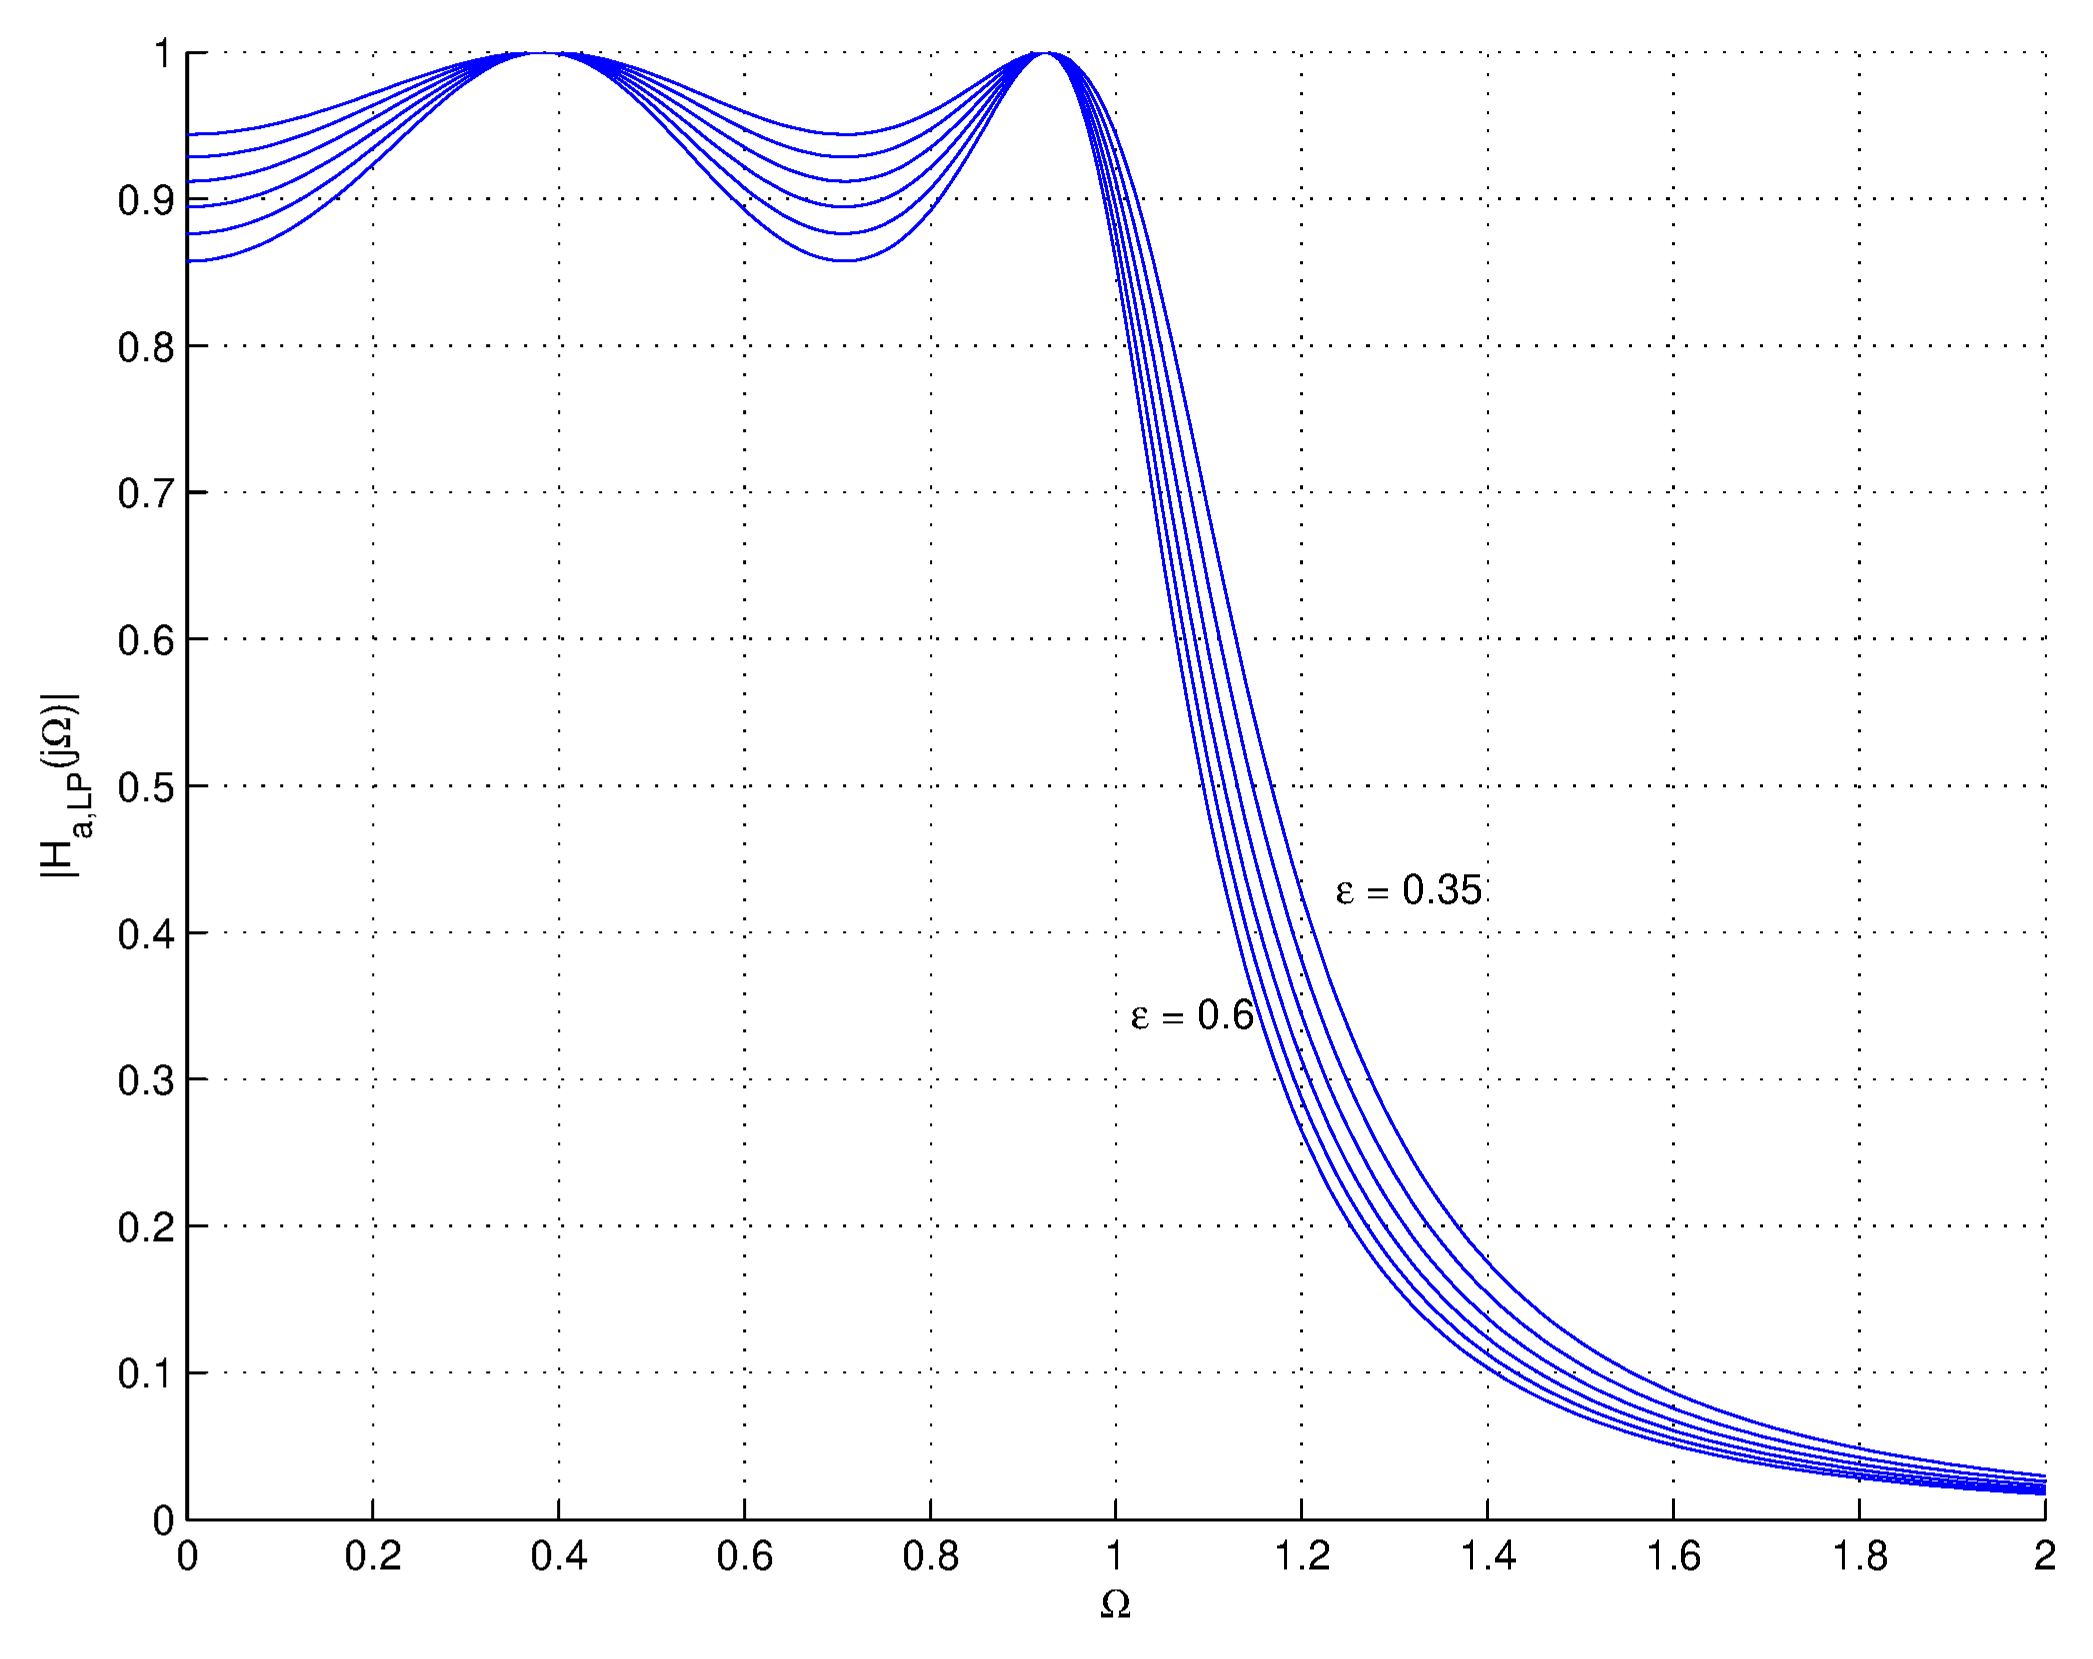
\includegraphics[width=\columnwidth]{figs/PNG/IIR/fig1.png}
\caption{The Analog Low-Pass Frequency Response for $0.35 \leq \epsilon \leq 0.6$}
\label{fig:fig1}
\end{figure}

\noindent{\em The Low Pass Chebyschev Filter:} 

\begin{equation}
\label{lpsqfinal}
\vert H_{a,LP}(j\Omega_L)\vert^2 = \frac{1}{1 + 0.16c_4^2(\Omega_L)}
\end{equation}
where,
\begin{equation}
c_4(x) = 8x^4 + 8x^2 + 1.	
\end{equation}
% The poles of the frequency response in (\ref{lpfirst}) lying in the left half plane are in general obtained as 
% $r_1\cos\phi_k + jr_2\sin \phi_k$, where
% \begin{eqnarray}
% \label{lppoles}
% \phi_k = \frac{\pi}{2} + \frac{(2k+1)\pi}{2N}, k = 0, 1, \dots, N-1 \nonumber \\
% r_1 = \frac{\beta^2 - 1}{2\beta}, r_2 = \frac{\beta^2 + 1}{2\beta}, \beta = \left[ \frac{\sqrt{1 + \epsilon^2} + 1}{\epsilon}\right]^{\frac{1}{N}}
% \end{eqnarray}
% Thus, for N even, 
The low-pass stable Chebyschev fiter, with a gain $G$ has the form:
\begin{equation}
\label{poleleft}
H_{a,LP}(s_L) = \frac{G_{LP}}{\prod_{k = 1}^{\frac{N}{2}-1}(s_L^2 - 2r_1\cos\phi_ks_L + r_1^2\cos^2\phi_k + r_2^2 \sin^2\phi_k)}
\end{equation}
Substituting $N = 4$, $\epsilon = 0.5$ and $H_{a,LP}(j) = \frac{1}{\sqrt{1+\epsilon^2}}$, from (\ref{poleleft}), we obtain 
\begin{equation}
\label{lpfinal}
H_{a,LP}(s_L) = \frac{0.3125}{s_L^4 + 1.1068s_L^3 + 1.6125s_L^2+0.9140s_L + 0.3366}
\end{equation}
In Figure \eqref{fig:fig2} we plot $|H(j\Omega)|$ using (\ref{lpsqfinal}) and (\ref{lpfinal}), thereby verifying that our low-pass Chebyschev filter design meets the specifications.
% \begin{itemize}
% \item The {\em analog  passband} frequencies are $\Omega_{p1} = 0.5095$, $\Omega_{p2} = 0.4142$
% \item The {\em analog  stopband} frequencies are $\Omega_{s1} = 0.5345$, $\Omega_{s2} = 0.3914$
% \end{itemize}
% \begin{itemize}



\begin{figure}[htbp] 
\centering
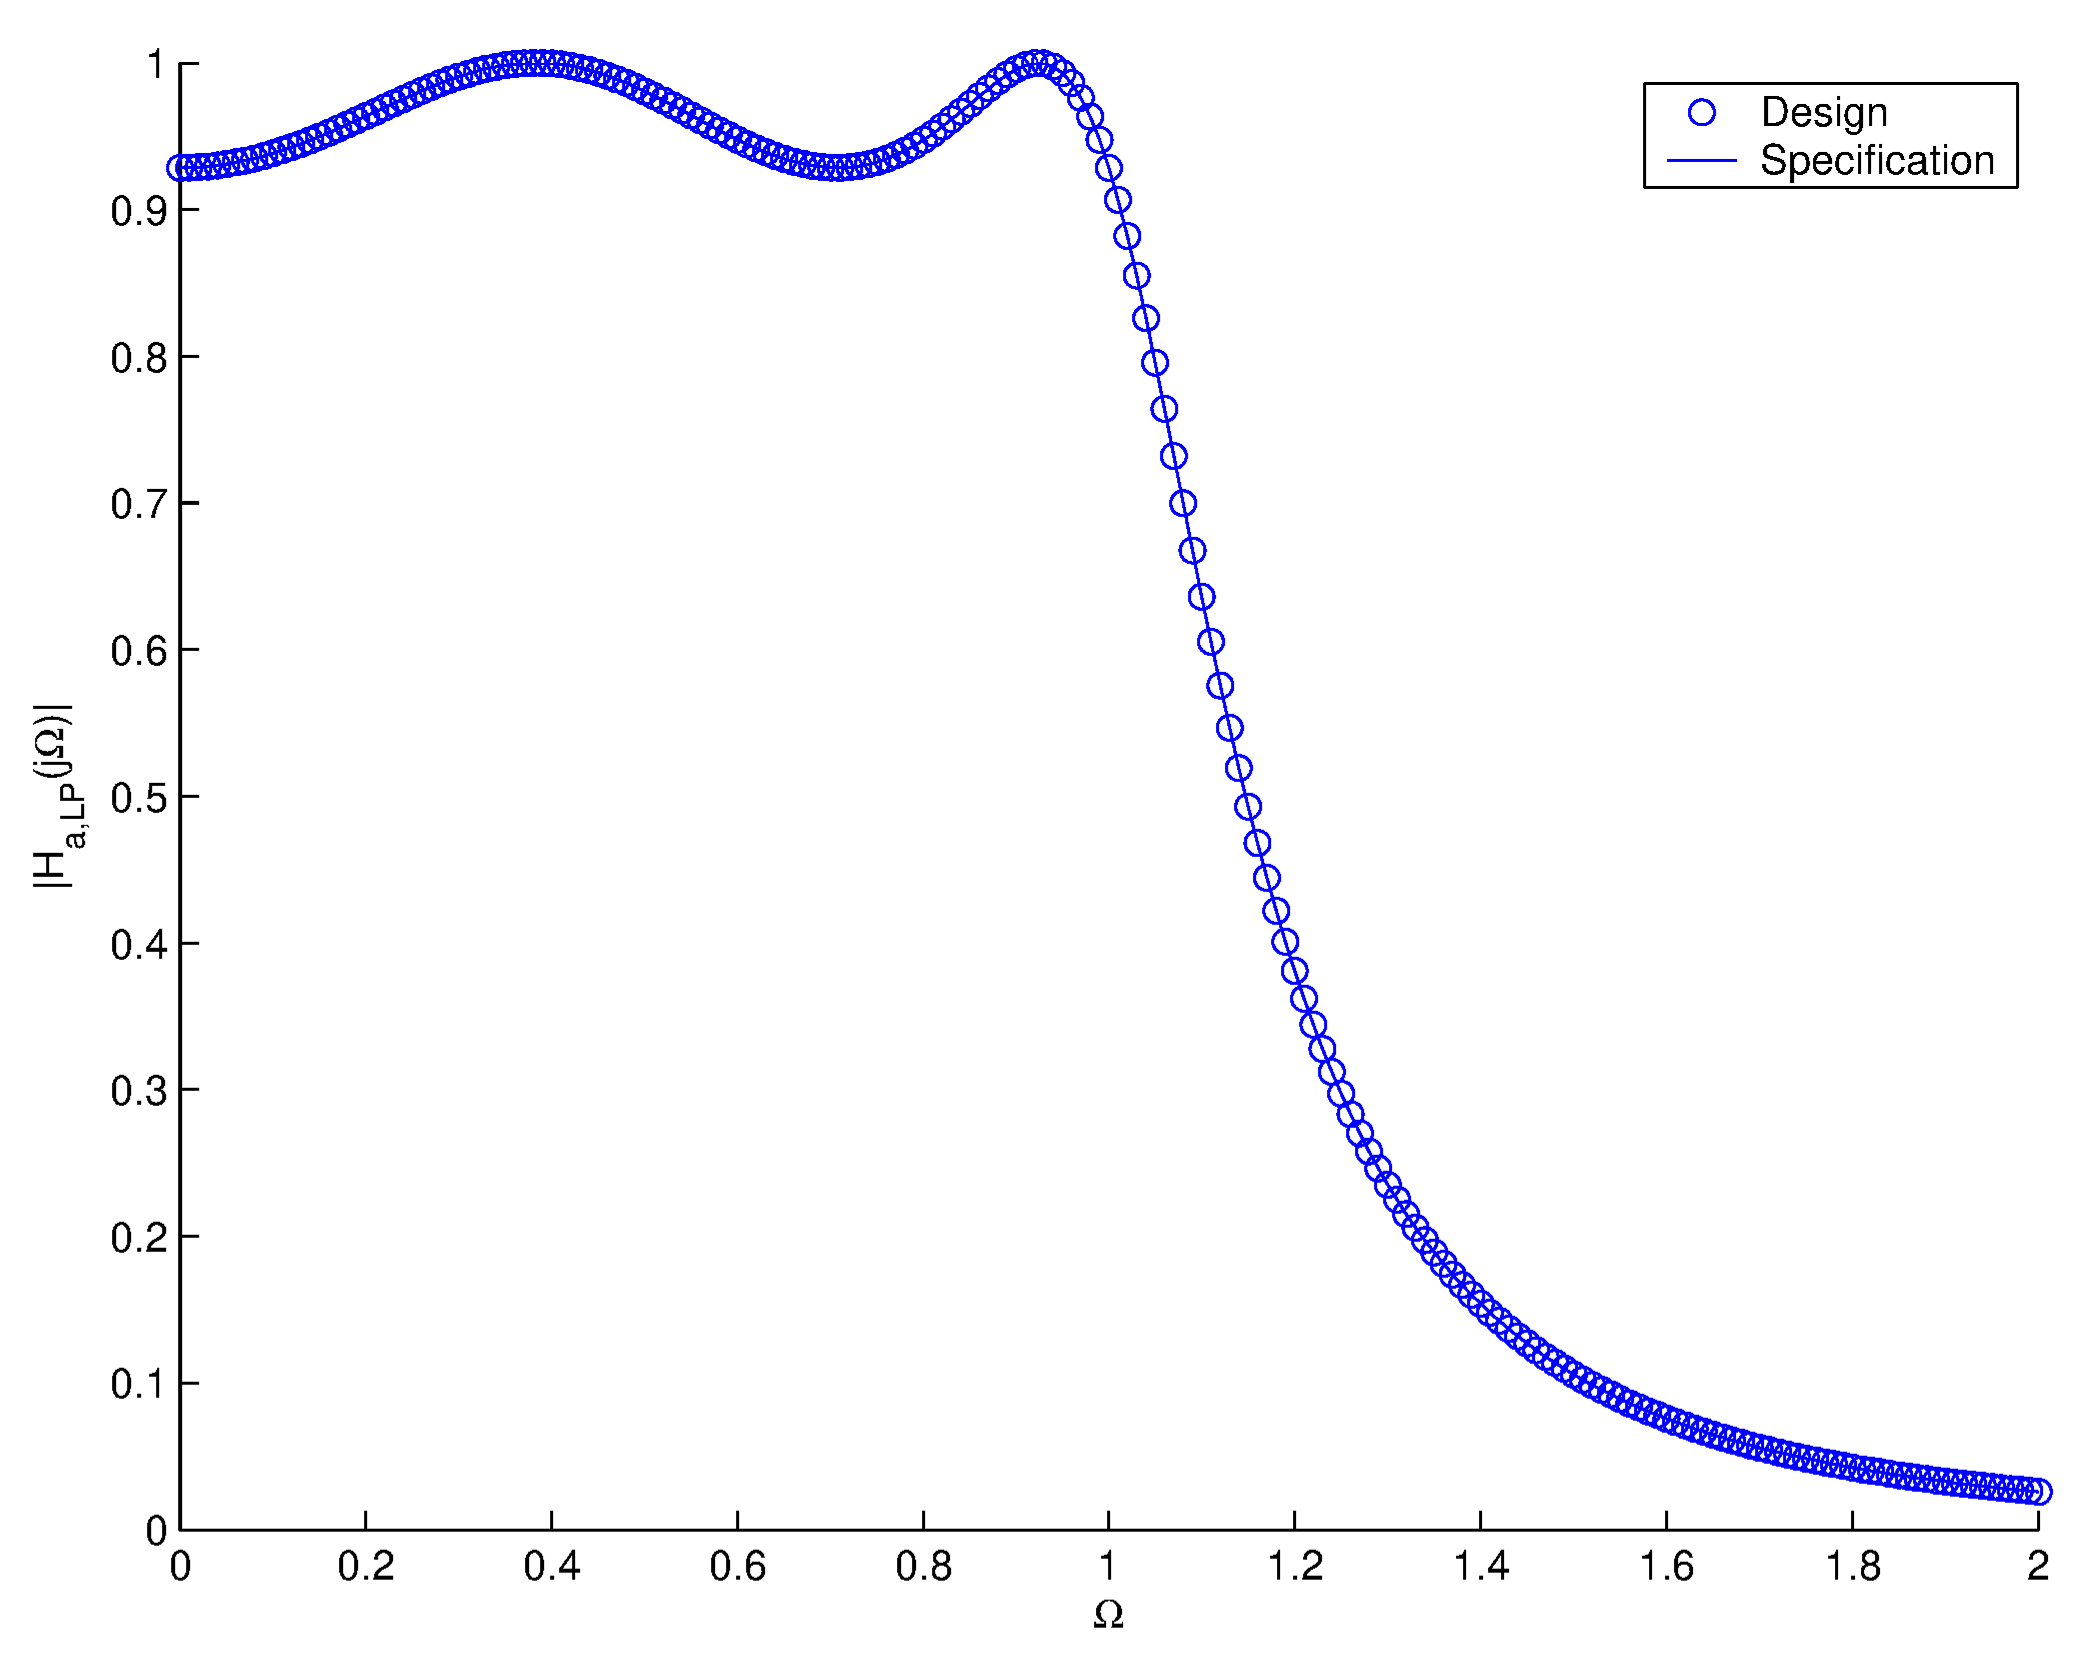
\includegraphics[width=1.1\columnwidth]{figs/PNG/IIR/fig2.png}
\caption{The magnitude response plots from the specifications in Equation \ref{lpsqfinal} and the design in Equation\eqref{lpfinal}}
\label{fig:fig2}
\end{figure}
 \begin{itemize}
\item The {\em analog  passband} frequencies are $\Omega_{p1} = 0.5095$, $\Omega_{p2} = 0.4142$
\item The {\em analog  stopband} frequencies are $\Omega_{s1} = 0.5345$, $\Omega_{s2} = 0.3914$
\item If $\Omega$ be the {\em analog bandpass} frequency and $\Omega_L$ be the corresponding {\em analog lowpass} frequency,
\begin{equation}
\Omega_L = \frac{\Omega^2 - \Omega_0^2}{B\Omega}.
\end{equation}

\item $\Omega_0 = \sqrt{\Omega_{p1}\Omega_{p2}} = 0.4594$ and $B = \Omega_{p1} - \Omega_{p2} = 0.0953$
\end{itemize}
\noindent{\em The Band Pass Chebyschev Filter:} 

The analog bandpass filter is obtained from (\ref{lpfinal}) by substituting
$s_L = \frac{s^2 + \Omega_0^2}{Bs}$.  Hence
\begin{equation}
H_{a,BP}(s) = G_{BP}H_{a,LP}(s_L)\vert_{s_L = \frac{s^2 + \Omega_0^2}{Bs}},
\end{equation}
where $G_{BP}$ is the gain of the bandpass filter.  After appropriate substitutions, and evaluating the gain 
such that $H_{a,BP}(j\Omega_{p1}) = 1$, we obtain
{\tiny
\begin{equation}
\label{bpfinal}
H_{a,BP}(s) = \frac{2.7776\times 10^{-5}s^4}{s^8+0.1055s^7+0.8589s^6+0.0676s^5+0.2735s^4+0.0143s^3+0.0383s^2+0.001s+0.002}
\end{equation}
}
In Figure \eqref{fig:fig3}, we plot $\vert H_{a,BP}(j\Omega)\vert$ as a function of $\Omega$ for both positve as
well as negative frequencies.  We find that the passband and stopband frequencies in the figure
match well with those obtained analytically through the bilinear transformation.

\begin{figure}[htbp] 
\centering
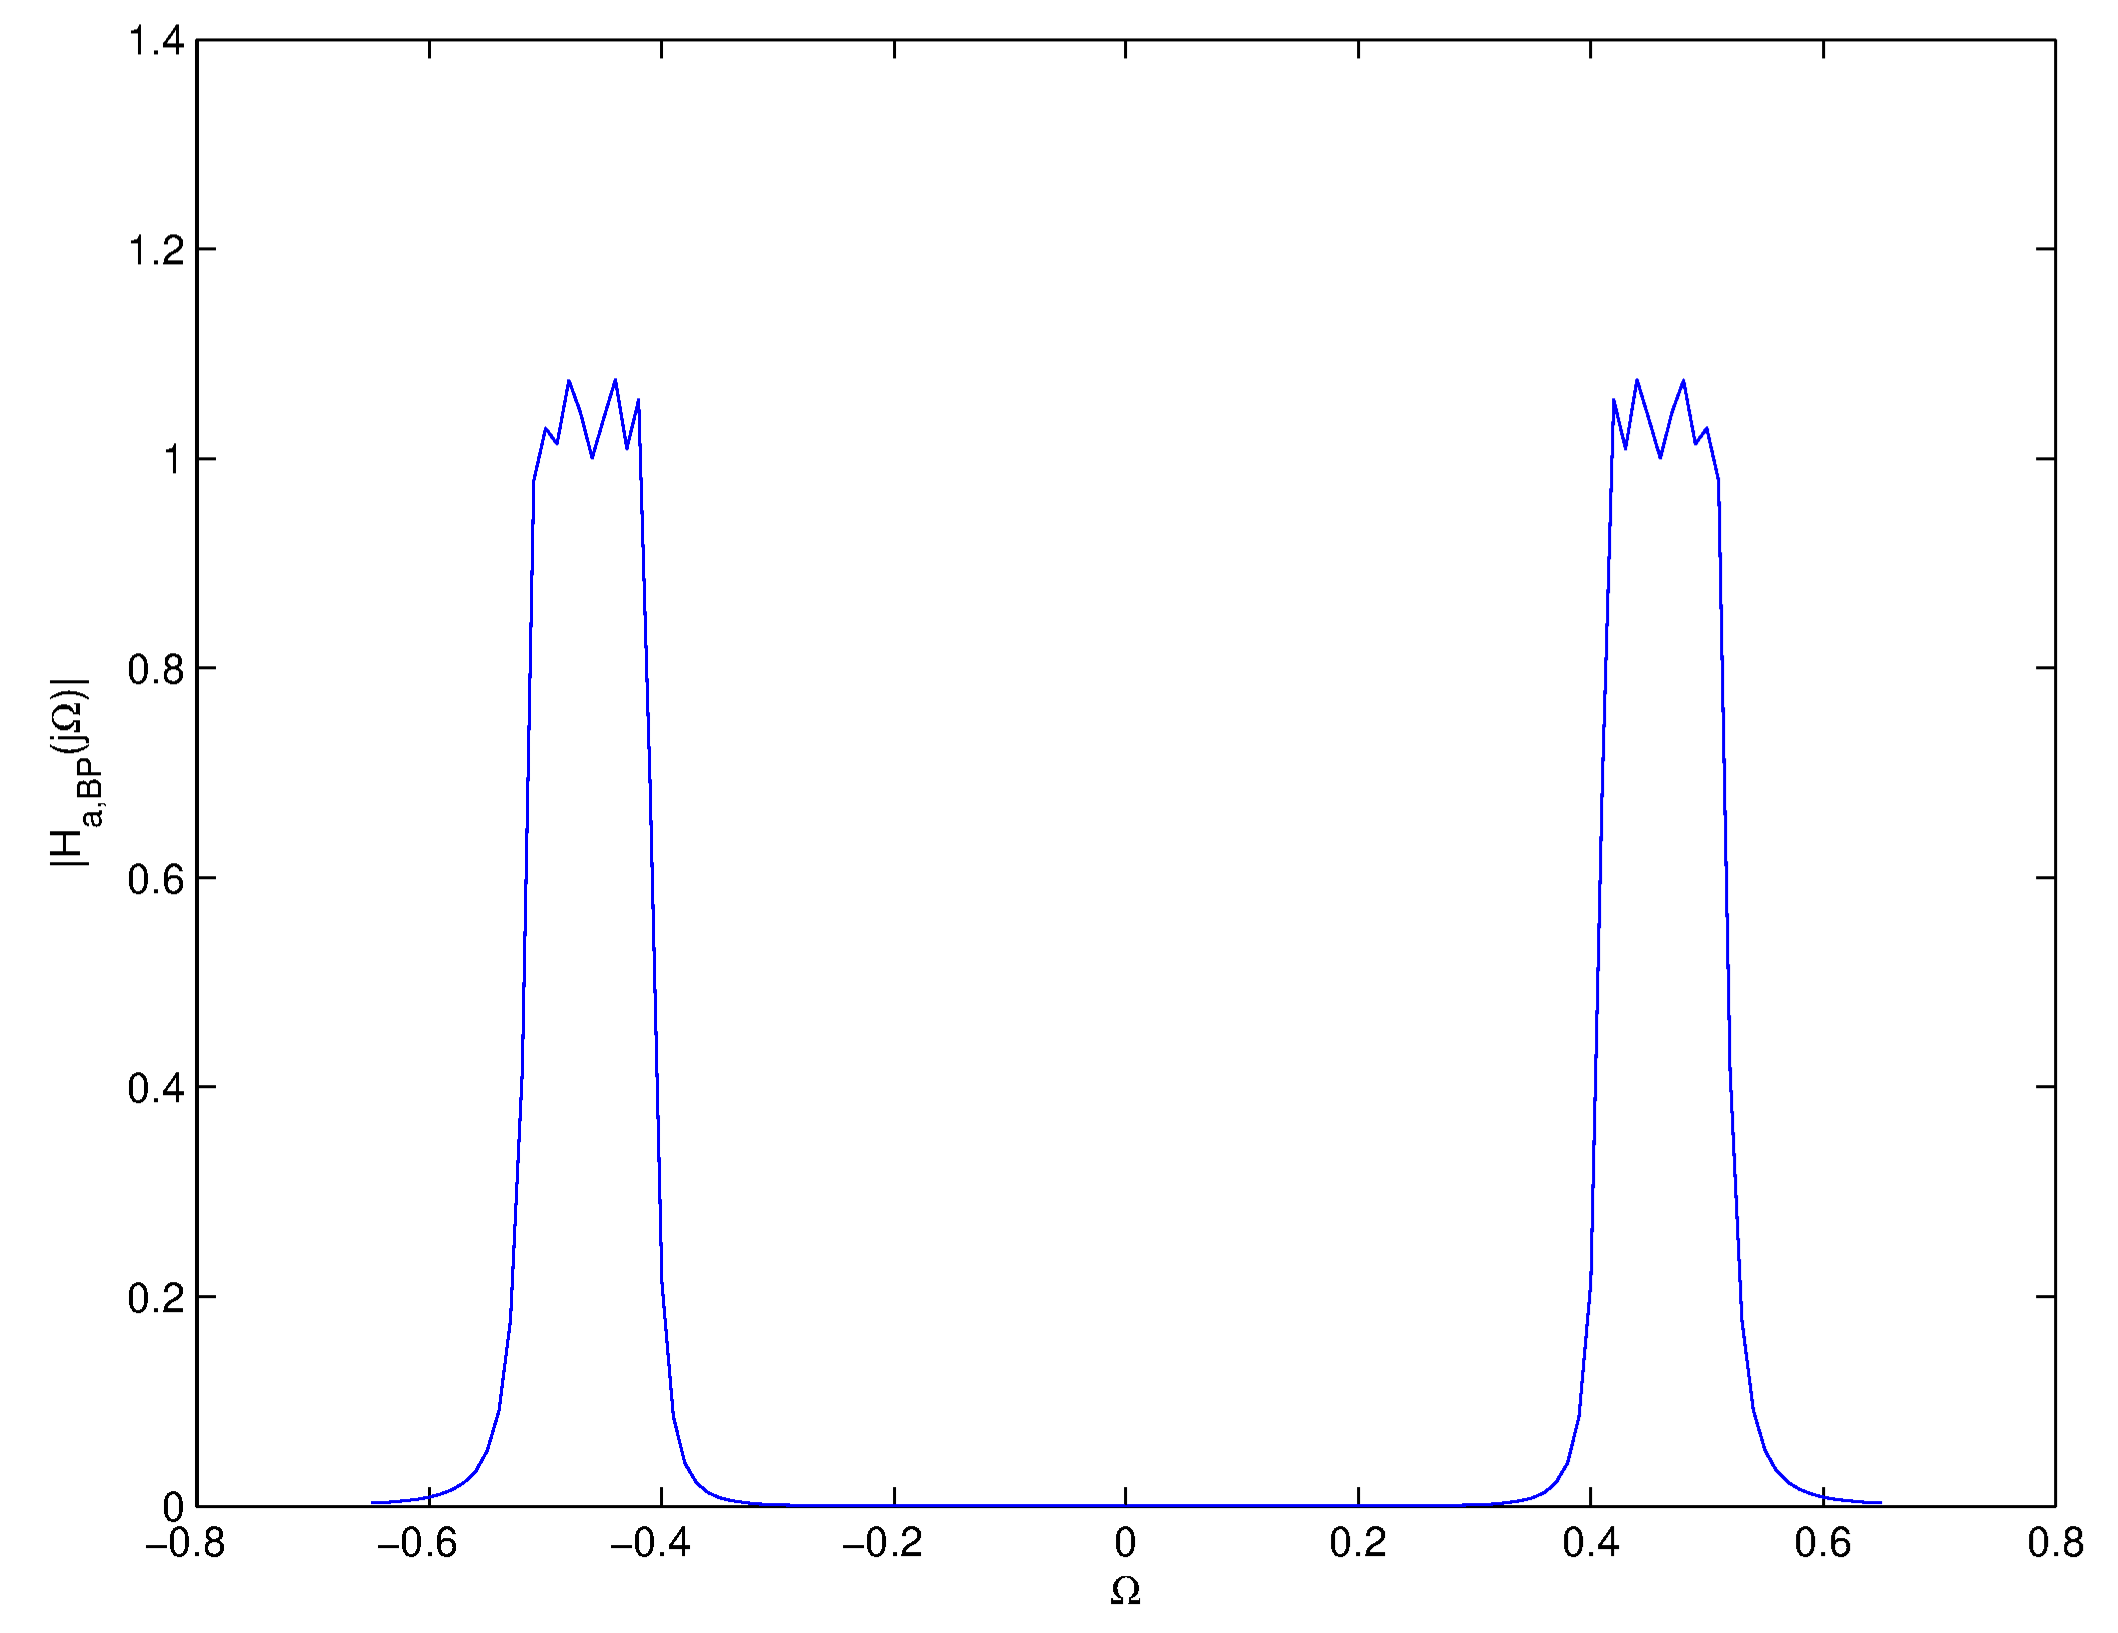
\includegraphics[width=\columnwidth]{figs/PNG/IIR/fig3.png}
\caption{The analog bandpass magnitude response plot from Equation \ref{bpfinal}}
\label{fig:fig3}
\end{figure}

\subsection{The Digital Filter}
% From the bilinear transformation, we obtain the digital bandpass filter from the corresponding analog filter as
% \begin{eqnarray}
% \label{analdig}
% H_{d,BP}(z) = GH_{a,BP}(s)\vert_{s = \frac{1-z^{-1}}{1 + z^{-1}}}
% \end{eqnarray}
% where $G$ is the gain of the digital filter.  From (\ref{bpfinal}) and (\ref{analdig}), we obtain

\begin{eqnarray}
H_{d,BP}(z) = G \frac{N(z)}{D(z)}
\end{eqnarray}
where, $G = 2.7776 \times 10^{-5}$,

\begin{eqnarray}
N(z)=  1 - 4 z^{-2} + 6 z^{-4} - 4z^{-6} + z^{-8} 
\end{eqnarray}
and
\begin{multline}
D(z) = 2.3609  -12.0002z^{-1} + 31.8772z^{-2}  -53.7495z^{-3}\\+  62.8086z^{-4} - 51.4634z^{-5}+   29.2231z^{-6}  -10.5329z^{-7} +   1.9842z^{-8}
\end{multline}
The plot of $|H_{d,BP}(z)|$ with respect to the normalized angular freqency (normalizing factor $\pi$) is available in Figure 4.  Again we
find that the passband and stopband frequencies meet the specifications well enough.

\begin{figure}[htbp] 
\centering
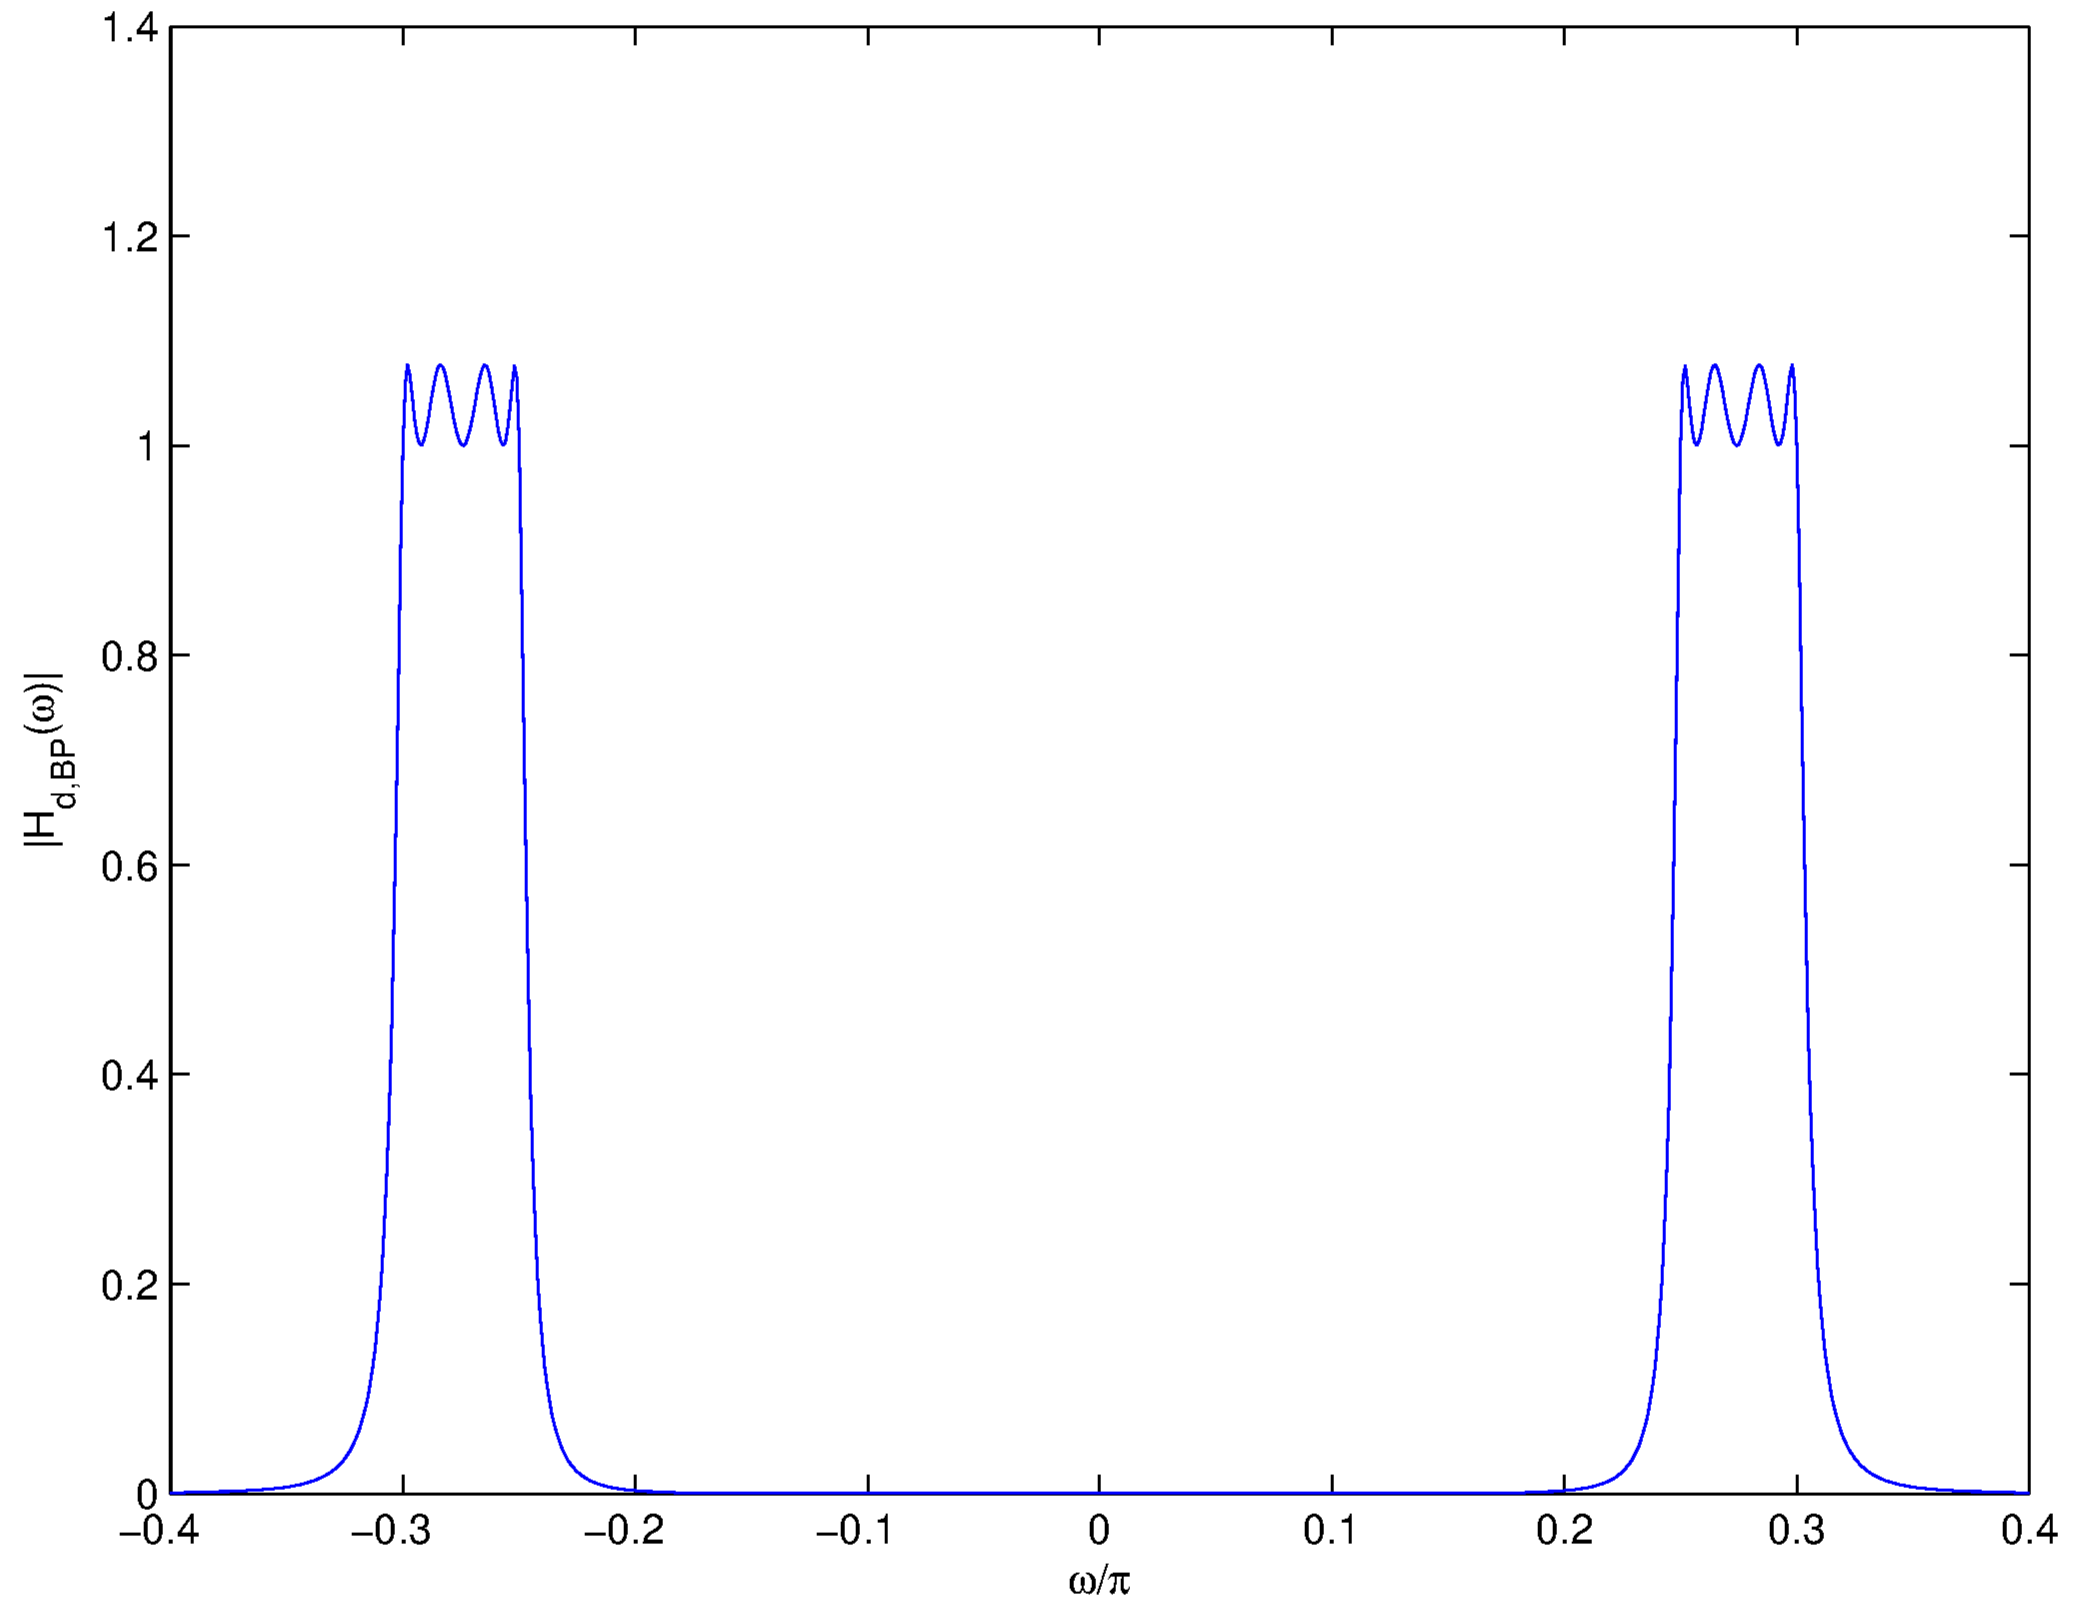
\includegraphics[width=\columnwidth]{figs/PNG/IIR/fig4.png}
\caption{The magnitude response of the bandpass digital filter designed to meet the given specifications}
\end{figure}
\section{FIR Filter Design}
We design the FIR filter by first obtaining the (non-causal) lowpass equivalent
using the Kaiser window and then converting it to a causal bandpass filter.

{\em FIR Filter Transfer Function Realization Using Kaiser Window:}

\begin{itemize}
\item The equivalent {\em lowpass} filter has {\em passband frequency $\omega_l = \frac{\omega_{p1} - \omega_{p2}}{2} = 0.025\pi$}.

\item The centre of the passband of the desired bandpass filter is $\omega_c = \frac{\omega_{p1} + \omega_{p2}}{2} = 0.275\pi$
\item For the given specifications, the {\em Kaiser} window reduces to the {\em rectangular} window of {\em length
$\geq 97$}.
\item The desired {\em lowpass filter impulse response}
\begin{eqnarray}
\label{firlpfinal}
h_{lp}(n) &=& \frac{\sin(\frac{n\pi}{40})}{n\pi} \hspace{2cm} -100 \leq n \leq 100 \nonumber \\
&=& 0, \hspace{4cm} \mbox{otherwise} \nonumber
\end{eqnarray}

\begin{figure}[htbp] 
\centering
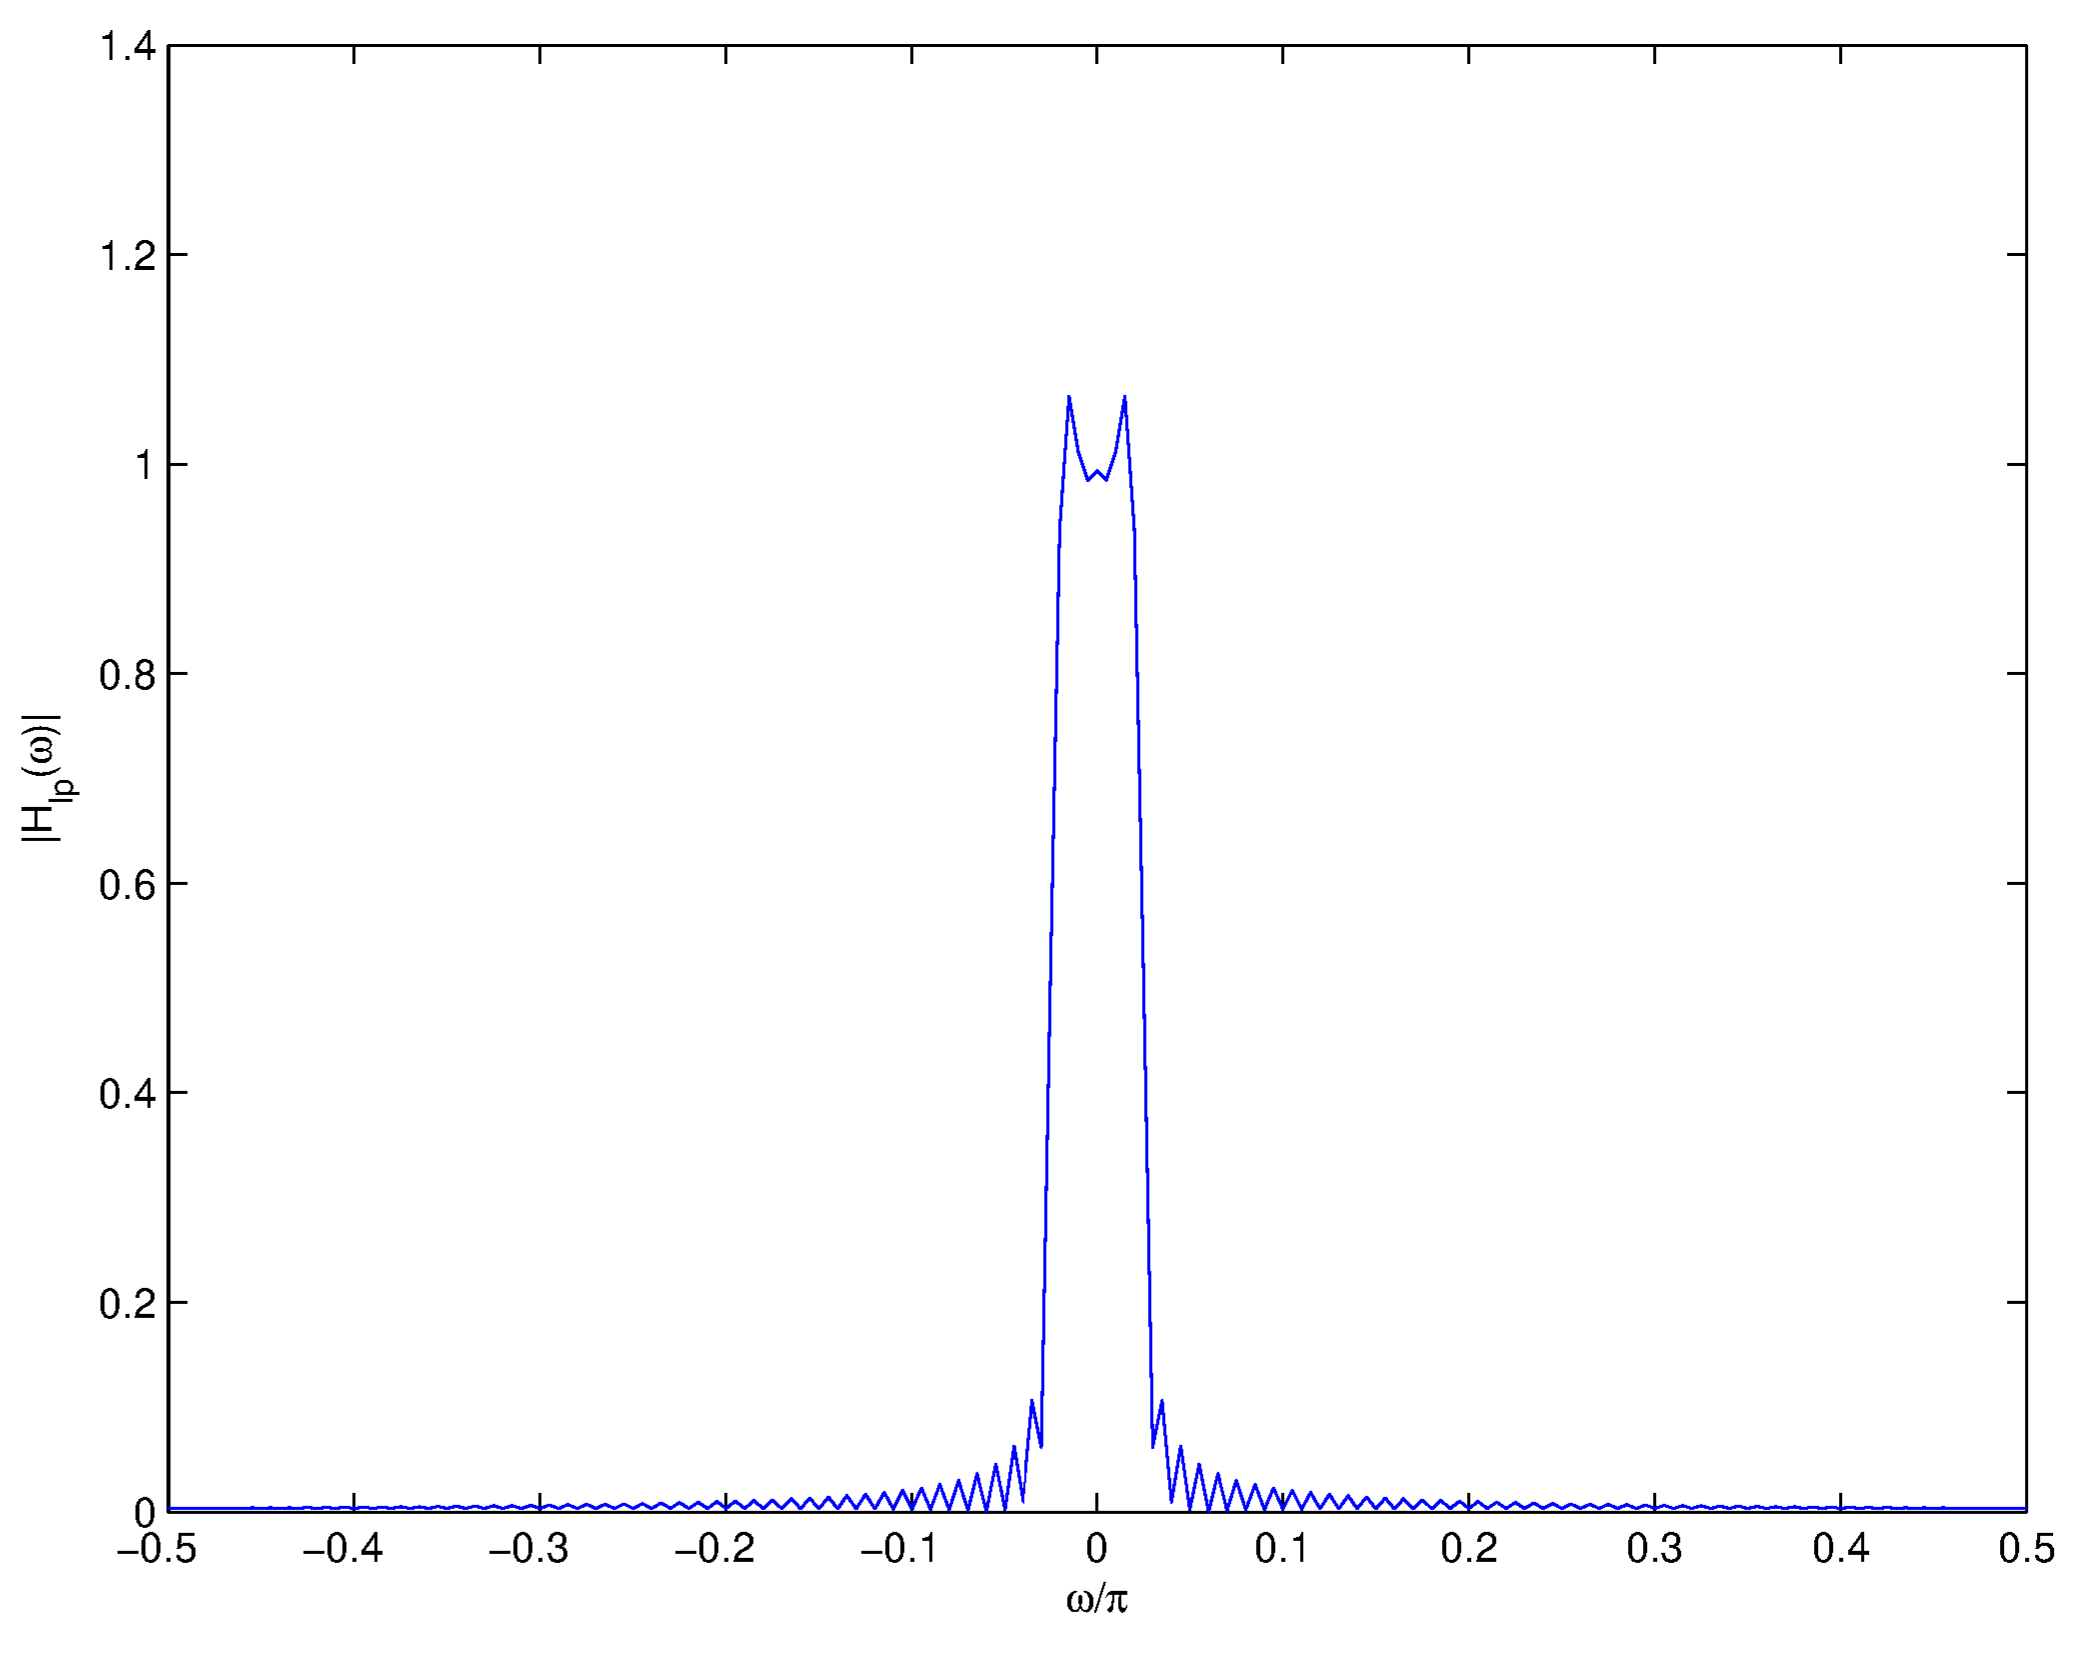
\includegraphics[width=\columnwidth]{figs/PNG/FIR/fig5.png}
\caption{The magnitude response of the FIR lowpass digital filter designed to meet the given specifications}
\label{fig:fig5}
\end{figure}

\item The desired {\em bandpass filter impulse response}
\begin{eqnarray}
\label{firbpfinal}
h_{bp}(n) &=& \frac{2\sin(\frac{n\pi}{40}) \cos(\frac{11n\pi}{40})}{n\pi} \hspace{1cm} -100 \leq n \leq 100 \nonumber \\
&=& 0, \hspace{4cm} \mbox{otherwise}\nonumber
\end{eqnarray}
\end{itemize}
\begin{figure}[htbp] 
\centering
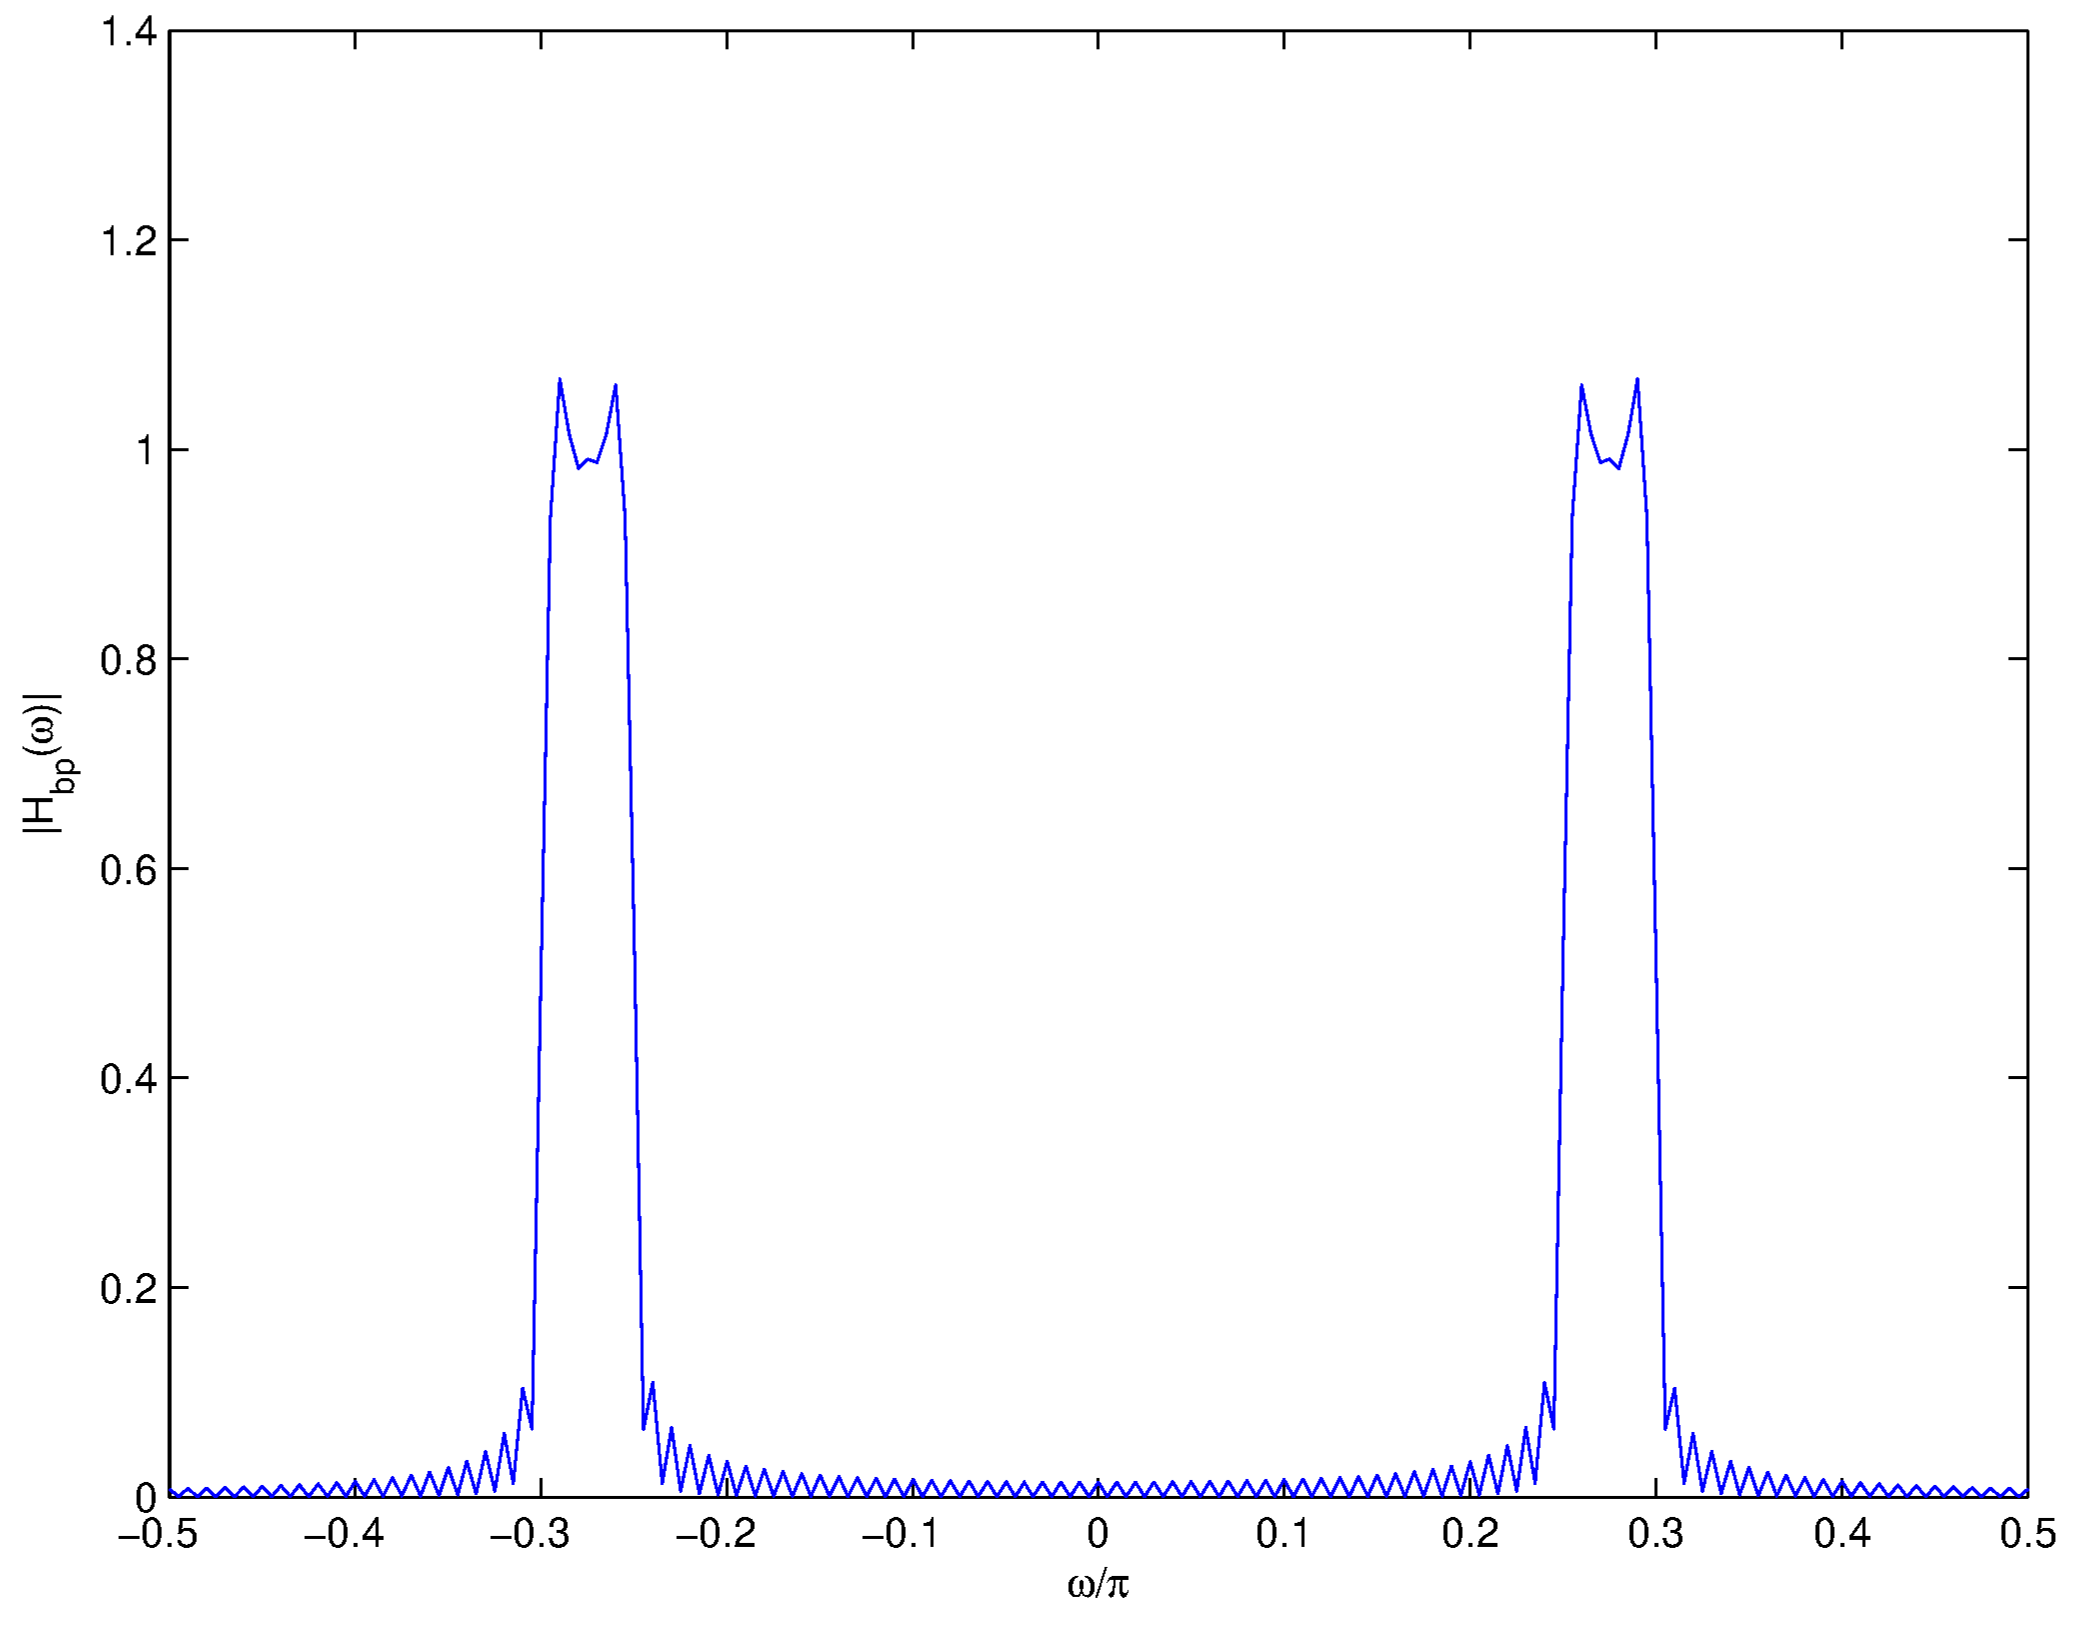
\includegraphics[width=\columnwidth]{figs/PNG/FIR/fig6.png}
\caption{The magnitude response of the FIR bandpass digital filter designed to meet the given specifications}
\label{fig:fig5}
\end{figure}
% \end{enumerate}
\end{document}l
